\documentclass[journal]{IEEEtran}

\ifCLASSINFOpdf
\else
   \usepackage[dvips]{graphicx}
\fi
\usepackage{url}
\usepackage{listings}
\usepackage[margin=1in]{geometry}
\usepackage{amsmath,amsthm,amssymb}
\usepackage[margin=1in]{geometry}
\usepackage{amsmath,amsthm,amssymb}
\usepackage[spanish]{babel} %Castellanización
\usepackage[T1]{fontenc} %escribe lo del teclado
\usepackage[utf8]{inputenc} %Reconoce algunos símbolos
\usepackage{lmodern} %optimiza algunas fuentes
\usepackage{graphicx}
\usepackage{blkarray}
\usepackage{amsmath}
\usepackage{algorithm}
\usepackage[noend]{algpseudocode}
\graphicspath{ {images/} }
\usepackage{hyperref} % Uso de links
\usepackage[options ]{algorithm2e}
\newcommand{\N}{\mathbb{N}}
\newcommand{\Z}{\mathbb{Z}}
 \usepackage{float}
\newenvironment{theorem}[2][Theorem]{\begin{trivlist}
\item[\hskip \labelsep {\bfseries #1}\hskip \labelsep {\bfseries #2.}]}{\end{trivlist}}
\newenvironment{lemma}[2][Lemma]{\begin{trivlist}
\item[\hskip \labelsep {\bfseries #1}\hskip \labelsep {\bfseries #2.}]}{\end{trivlist}}
\newenvironment{exercise}[2][Exercise]{\begin{trivlist}
\item[\hskip \labelsep {\bfseries #1}\hskip \labelsep {\bfseries #2.}]}{\end{trivlist}}
\newenvironment{problem}[2][Problem]{\begin{trivlist}
\item[\hskip \labelsep {\bfseries #1}\hskip \labelsep {\bfseries #2.}]}{\end{trivlist}}
\newenvironment{question}[2][Question]{\begin{trivlist}
\item[\hskip \labelsep {\bfseries #1}\hskip \labelsep {\bfseries #2.}]}{\end{trivlist}}
\newenvironment{corollary}[2][Corollary]{\begin{trivlist}
\item[\hskip \labelsep {\bfseries #1}\hskip \labelsep {\bfseries #2.}]}{\end{trivlist}}
\newcommand*{\defeq}{\stackrel{\text{def}}{=}}
\newenvironment{solution}{\begin{proof}[Solution]}{\end{proof}}
\hyphenation{op-tical net-works semi-conduc-tor}

\usepackage{graphicx}


\usepackage{amsmath}
\usepackage{algorithm}
\usepackage[noend]{algpseudocode}

\makeatletter
\def\BState{\State\hskip-\ALG@thistlm}
\makeatother

\begin{document}

\title{Tarea 2: Optimización - Convexidad y Descenso de Gradiente}

\author{Oscar Esaú Peralta Rosales, \IEEEmembership{Maestría en Ciencias de la Computación}}

\markboth{Febrero 2020}
{Shell \MakeLowercase{\textit{et al.}}: Bare Demo of IEEEtran.cls for IEEE Journals}
\maketitle

\begin{abstract}
A continuación se presentan la solución a 3 ejercicios en materia de Convexidad sobre conjuntos y funciones. Dado a esta misma caracteristica de convexidad presente sobre funciones, nos permite realizar procesos de optimización sobre estás mismas. En especial se remota el algoritmo de Descenso de Gradiente y se muestra los distintos resultados usando 3 formas de obtener el tamaño de paso y criterios de parada.
\end{abstract}

\begin{IEEEkeywords}
Descenso del gradiente, Convexidad
\end{IEEEkeywords}


\IEEEpeerreviewmaketitle



\section{Introduction}

\IEEEPARstart{E}{l} método del descenso del gradiente es un algoritmo de optimización sobre funciones que presentan caracteristicas de convexidad sobre cierto intervalo y así poder identicar mínimos y máximos en esta. \\

Para poder identificar dichos minimos o máximos se hace uso de la gradiente de la función, puesto que esta nos representa la dirección de máximo crecimiento y por tanto moverse en dicha dirección o en sentido contrario nos permite minimzar y maximizar la función.

En la primer sección se presentan la solución a 3 problemas con respecto a Convexidad de conjuntos y funciones. La segunda sección contiene el proceso y resultados de la implementación del Algoritmo de Descenso de Gradiente.

\subsection{Problemas}

\subsubsection{Problema 1}

El conjunto $S = \{ a \in \mathcal{R}^k | p(0)=1, |p(t)| \le 1 para un t \in [\alpha, \beta] \}$ donde $a = [a_1, ..., a_1]^T$ y $p(t) = a_1 + a_2t+ ... + a_kt^{k-1}$, ¿Es convexo?.

\textbf{Solución}

Sean $a, b \in S$ dos vectores y $\mu \in [0,1]$ por probar que $\mu a + (1-\mu)b \in S$ es verdadera.

Cómo $a, b \in S$ entonces existe un $t \in (\alpha, \beta)$ tal que $p(t) = a_1 + a_2t + ... + a_kt^{k-1}$ y $p(t) = b_1 + b_2t + ... + b_kt^{k-1}$.
Además notemos que si $p(0) = 1$ entonces $a_1 = 1$ y $b_1=1$.

Comprobemos que si $\mu a + (1-\mu)b \in S$ entonces $p_{ab}(t) = (\mu a_1 + (1-\mu)b_1) + (\mu a_2 + (1-\mu)b_2)t + ... + (\mu a_k + (1-\mu)b_k)t^{k-1r}$ evualuado en cero es 1.

$p_{ab}(t) = (\mu a_1 + (1-\mu)b_1) + (\mu a_2 + (1-\mu)b_2)t + ... + (\mu a_k + (1-\mu)b_k)t^{k-1r}$

$p_{ab}(0) = (\mu a_1 + (1-\mu)b_1) + (\mu a_2 + (1-\mu)b_2)*0 + ... + (\mu a_k + (1-\mu)b_k)*0 $

$p_{ab}(0) = (\mu a_1 + (1-\mu)b_1) = 1 + \mu a_1 -\mu b_1$

Cómo $a_1 = 1$ y $b_1=1$, entonces $p_{ab}(0) = 1$. Por otro lado como $|p(t)| \le 1$ entonces demostremos $|p_{ab}(t)| \le 1$, luego

$|p_{ab}(t)| = |(\mu a_1 + (1-\mu)b_1) + (\mu a_2 + (1-\mu)b_2)t + ... + (\mu a_k + (1-\mu)b_k)t^{k-1r}|$

$|p_{ab}(t)| = |\mu a_1 + (1-\mu)b_1 + \mu a_2 t + (1-\mu)b_2 t + ... + \mu a_k t^{k-1r} + (1-\mu)b_k t^{k-1r}|$

$|p_{ab}(t)| = |\mu a_1 + \mu a_2 t +...+ \mu a_k t^{k-1r} + (1-\mu)b_1 + (1-\mu)b_2 t +...+ (1-\mu)b_k t^{k-1r}|$

$|p_{ab}(t)| = |\mu (a_1 + a_2 t +...+ a_k t^{k-1r}) + (1-\mu) (b_1 + b_2 t +...+ b_k t^{k-1r})|$

$|p_{ab}(t)| \le \mu |a_1 + a_2 t +...+ a_k t^{k-1r}| + (1-\mu) |b_1 + b_2 t +...+ b_k t^{k-1r}|$

$|p_{ab}(t)| \le \mu |p(t)| + (1-\mu) |p(t)|$

Como $|p(t)| \le 1$ y $\mu \in [0,1]$ entonces $|p_{ab}(t)| \le 1$. Así $\mu a + (1-\mu)b \in S$ es verdadero y $S$ es convexo.

\subsubsection{Problema 2}

Suponga que *f* es convexa, $\lambda_1 > 0$, $\lambda_2 \le 0$ con $\lambda_1+\lambda_2 = 1$, y sean $x_1,x_2 \in dom\ f$. Muestre que la desigualdad $f(\lambda_1x_!+\lambda_2x_2) \ \ge \lambda_1f(x_1) + \lambda_2f(x_2)$ siempre se cumple.

\textbf{Solución}

Notemos que $\lambda_1 = 1 - \lambda_2$, como $\lambda_2 \le 0$ entonces $\lambda_1 \ge 1$ y dividiendo por $lambda_1$ tenemos que $1 \ge \frac{1}{\lambda_1}$ y como $\lambda_1 \ge 1$ entonces $0 < \frac{1}{\lambda_1} \le 1$. Sea $a$ y $b$ dos puntos en el dominio de $f$ y un $\alpha = \frac{1}{\lambda_1} \in (0, 1]$, luego como $f$ es convexa tenemos que

$f(\frac{1}{\lambda_1}a + (1- \frac{1}{\lambda_1})b) \le \frac{1}{\lambda_1}f(a) + (1 - \frac{1}{\lambda_1})f(b)$

$\lambda_1 f(\frac{1}{\lambda_1}a + (1- \frac{1}{\lambda_1})b) \le f(a) + (\lambda_1 - 1)f(b)$

$\lambda_1 f(\frac{1}{\lambda_1}a + (1- \frac{1}{\lambda_1})b) \le f(a) - \lambda_2f(b)$

$f(a) \ge \lambda_1 f(\frac{1}{\lambda_1}a + (1- \frac{1}{\lambda_1})b)+ \lambda_2f(b)$

Tomemos $a = \lambda_1x_1 + \lambda_2x_2$ y $b = x_2$

$f(\lambda_1x_1 + \lambda_2x_2) \ge \lambda_1 f(\frac{\lambda_1x_1 + \lambda_2x_2}{\lambda_1} + (1- \frac{1}{\lambda_1})x_2)+ \lambda_2f(x_2)$

$f(\lambda_1x_1 + \lambda_2x_2) \ge \lambda_1 f(x_1 + \frac{\lambda_2}{\lambda_1}x_2 + (x_2 - \frac{x_2}{\lambda_1}))+ \lambda_2f(x_2)$

$f(\lambda_1x_1 + \lambda_2x_2) \ge \lambda_1 f(x_1 + x_2 (\frac{\lambda_2 - 1}{\lambda_1} + 1))+ \lambda_2f(x_2)$

$f(\lambda_1x_1 + \lambda_2x_2) \ge \lambda_1 f(x_1 + x_2 (\frac{\lambda_2 - 1}{\lambda_1} + {\frac{\lambda_1}{\lambda_1}}))+ \lambda_2f(x_2)$

$f(\lambda_1x_1 + \lambda_2x_2) \ge \lambda_1 f(x_1 + x_2 (\frac{\lambda_2 + \lambda_1 - 1}{\lambda_1}))+ \lambda_2f(x_2)$

Como $\lambda_1 + \lambda_2 = 1$

$f(\lambda_1x_1 + \lambda_2x_2) \ge \lambda_1 f(x_1 + x_2 (\frac{0}{\lambda_1}))+ \lambda_2f(x_2)$

y así

$f(\lambda_1x_1 + \lambda_2x_2) \ge \lambda_1 f(x_1)+ \lambda_2f(x_2)$

\subsubsection{Problema 3}

Muestre que la función $f:\mathcal{R}^n \rightarrow \mathcal{R}$, $f(x) = -\exp(-g(x))$ es convexa, donde $g:\mathcal{R}^n \rightarrow \mathcal{R}$ tiene un dominio convexo y cumple

$$
\begin{pmatrix}
	\nabla^2g(x) & \nabla g(x)\\
	\nabla ^ T g(x) & 1\\
\end{pmatrix} \ge 0
$$

para $x \in dom\ g$

\textbf{Solución}

$f$ es convexa si su Hessiano asociado es semidefinido positivo o positivo. Así procedamos a calcularlo.

$ f(x) = -\exp(-g(x)) $

$ \nabla_xf(x) = \exp(-g(x)) \nabla g(x) $

$ \nabla_x^2 f(x) = \exp(-g(x)) \nabla^2 g(x) - \nabla g(x) \exp(-g(x)) \nabla^T g(x) $

$ \nabla_x^2 f(x) = \exp(-g(x)) \Big (\nabla^2 g(x) - \nabla g(x) \nabla^T g(x) \Big) $

Notemos que $\exp(-g(x))$ es positivo solonos falta comprobar que $\nabla^2 g(x) - \nabla g(x) \nabla^T g(x)$ sea una matriz definida positiva. Por otro lado la matriz provista anteriormente es semidefinida positiva y por tanto su determinante debe ser mayor o igual a cero
$$
det \begin{pmatrix}
	\nabla^2g(x) & \nabla g(x)\\
	\nabla ^ T g(x) & 1\\
\end{pmatrix} = \nabla^2g(x) - \nabla g(x) \nabla ^ T g(x) \ge 0
$$

por tanto

$ \nabla_x^2 f(x) = \exp(-g(x)) \big (\nabla^2 g(x) - \nabla g(x) \nabla^T g(x) \big) >=0 $

y así, $f$ es una función convexa.

\section{Metodología}

\subsection{Implementación del algoritmo de descenso de gradiente}

La implementación del algoritmo de Descenso de Gradiente fue implementado (en Python) en base al siguiente pseudocódigo.

% \begin{figure}[H]
    \centering
    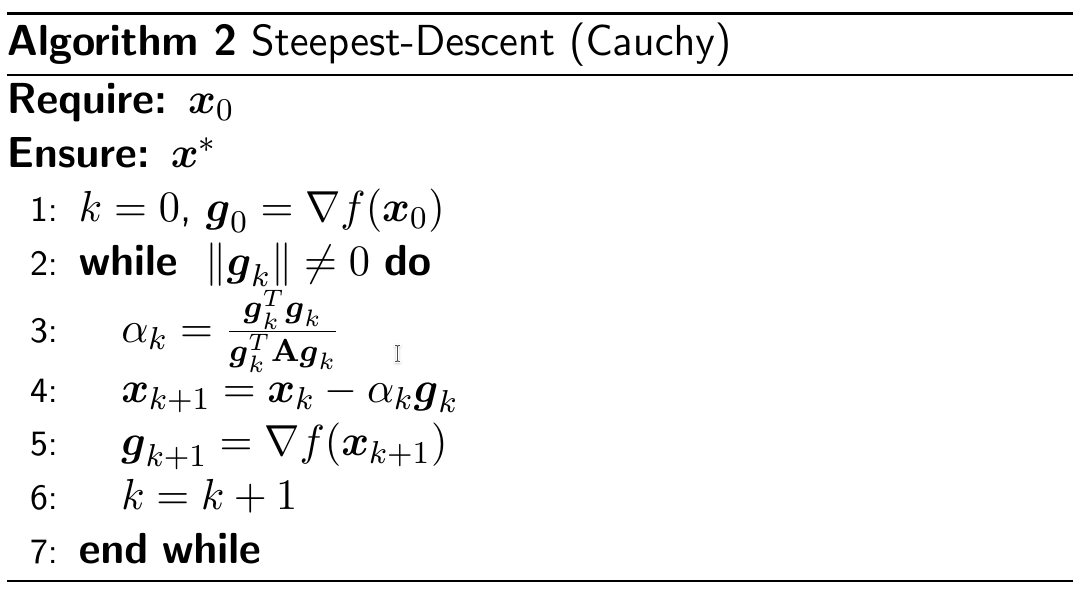
\includegraphics[scale=0.28]{1.png}
    % \caption{}
    \label{k}
% \end{figure}

Se implementaron 3 criterios para el cálculo del tamaño de paso:

\begin{itemize}
    \item Tamaño de paso fijo
    \item Tamaño de paso adaptable
    \item Tamaño de paso mediante backtracking
\end{itemize}

El tamaño de paso fijo, es seleccionado por el usuario y es invariante durante el proceso. El tamaño de paso adaptable es calculado mediante
$$
a_k = \frac{g_k^T g_k}{g_k^T H g_k}
$$

donde $H$ es la matriz Hessiana de la función a optimizar. El tamaño de paso calculado mediante backtraking se calcula como:

\lstset{language=Python}
\lstset{frame=lines}
\lstset{caption={Algoritmo del método de descenso del gradiente}}
\lstset{label={lst:code_direct}}
\lstset{basicstyle=\footnotesize}
\begin{lstlisting}
mientras f(x_k - alpha * gradiente_k) >
    f(x_k) + c1 * gradiente @ gradiente:
    alpha *= ro
\end{lstlisting}

Dónde $c1$ es una constante bastante pequeña y $ro$ es una constante que indica el decremento de $alpha$.

Se implementaron 3 criterios de paro para el algoritmo:

\begin{itemize}
    \item $ \frac{||x_{k+1}- x_k||}{max(1, ||x_k||)} < tol_x $
    \item $ \frac{||f(x_{k+1}) - f(x_k)||}{max(1, ||f(x_k)||)} < tol_f $
    \item $||\nabla f(x_k)|| < tol_g$
\end{itemize}

Donde $tol_x$, $tol_g$ y $tol_f$ son constantes de tolerancia para los 3 criterios anteriores.

Las pruebas fueron realizadas con 3 distintas funciones

\begin{itemize}
    \item Rosembrock, n = 2
    \item Rosembrock, n = 100
    \item Wood Function
\end{itemize}

\section{Resultados}

A continuación se presentan las tablas y figuras de resultados de las distintas ejecuciones.

\subsection{Resultados para la función de Rosembrock, n=2}

\begin{table}[H]
\begin{tabular}{@{}llll@{}}
k & $||x\_{k+1}-x_k||$ & $||\nabla f(x_k)||$ & $f(x_k)$ \\
1  &  1.547798E-01 &  2.328677E+02   &  -3.916000E+01  \\
2  &  2.784227E-02 &  3.094498E+01   &  -1.581861E+00  \\
3  &  1.075694E-02 &  1.948900E+00   &  4.745193E+00  \\
4668  &  3.813868E-11 &  1.637949E-09   &  -3.967826E-10 \\
4669  &  1.638340E-12 &  7.034957E-11   &  -3.076428E-11  \\
4670  &  3.090265E-11 &  1.338410E-09   &  -3.244516E-10
\end{tabular}
\caption{Cuadro comparativo de los criterios de paro y convergencia de la función con tamaño de paso adaptable}
\end{table}

\begin{figure}[H]
    \centering
    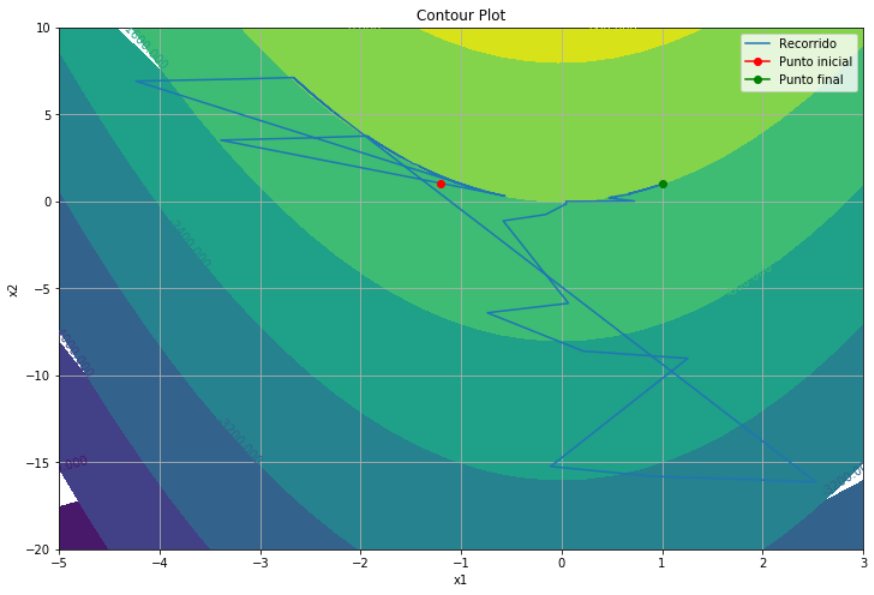
\includegraphics[scale=0.25]{2.png}
    \caption{Gráfico de contornos y convergencia para tamaño de paso adaptable}
    \label{k}
\end{figure}


\begin{table}[H]
\begin{tabular}{@{}llll@{}}
k & $||x\_{k+1}-x_k||$ & $||\nabla f(x_k)||$ & $f(x_k)$ \\
1  &  1.145760E+00 &  1.338602E+04   &  -1.096000E+03  \\
2  &  8.254502E-01 &  4.111110E+03   &  -5.300356E+02  \\
3  &  6.425282E-01 &  1.300948E+03   &  -2.748457E+02  \\
10000  &  7.740560E-08 &  3.874305E-05   &  -1.841706E-05 \\
10001  &  7.850808E-08 &  3.929487E-05   &  -6.087296E-06  \\
10002  &  7.728221E-08 &  3.868129E-05   &  -1.838770E-05
\end{tabular}
\caption{Cuadro comparativo de los criterios de paro y convergencia de la función con tamaño de paso fijo=0.001}
\end{table}

\begin{figure}[H]
    \centering
    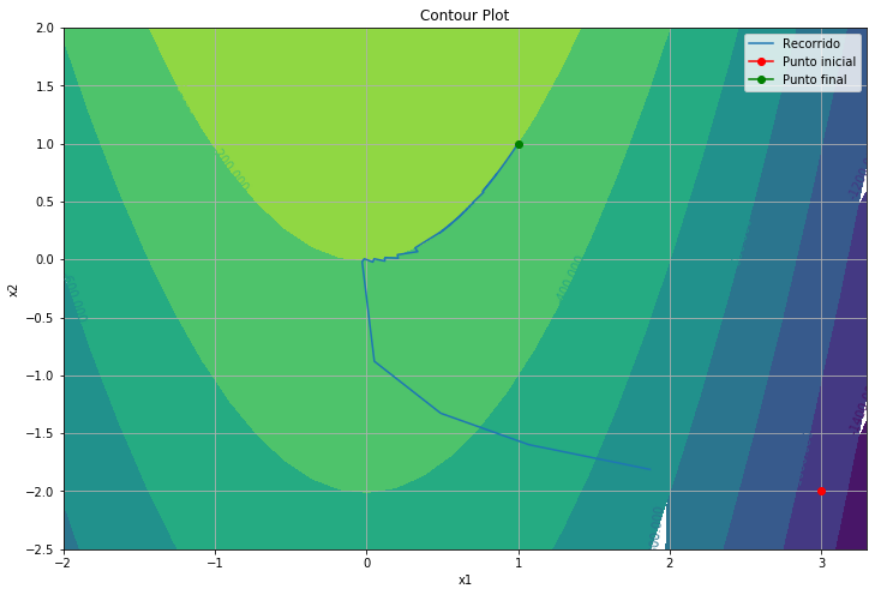
\includegraphics[scale=0.25]{3.png}
    \caption{Gráfico de contornos y convergencia para tamaño de paso fijo = 0.001}
    \label{k}
\end{figure}

\begin{table}[H]
\begin{tabular}{@{}llll@{}}
k & $||x\_{k+1}-x_k||$ & $||\nabla f(x_k)||$ & $f(x_k)$ \\
1  &  1.145760E+00 &  1.338602E+04   &  -1.096000E+03  \\
2  &  8.254502E-01 &  4.111110E+03   &  -5.300356E+02  \\
3  &  6.425282E-01 &  1.300948E+03   &  -2.748457E+02  \\
10000  &  7.740560E-08 &  3.874305E-05   &  -1.841706E-05 \\
10001  &  7.850808E-08 &  3.929487E-05   &  -6.087296E-06  \\
10002  &  7.728221E-08 &  3.868129E-05   &  -1.838770E-05
\end{tabular}
\caption{Cuadro comparativo de los criterios de paro y convergencia de la función con tamaño de paso por backtracking}
\end{table}

\begin{figure}[H]
    \centering
    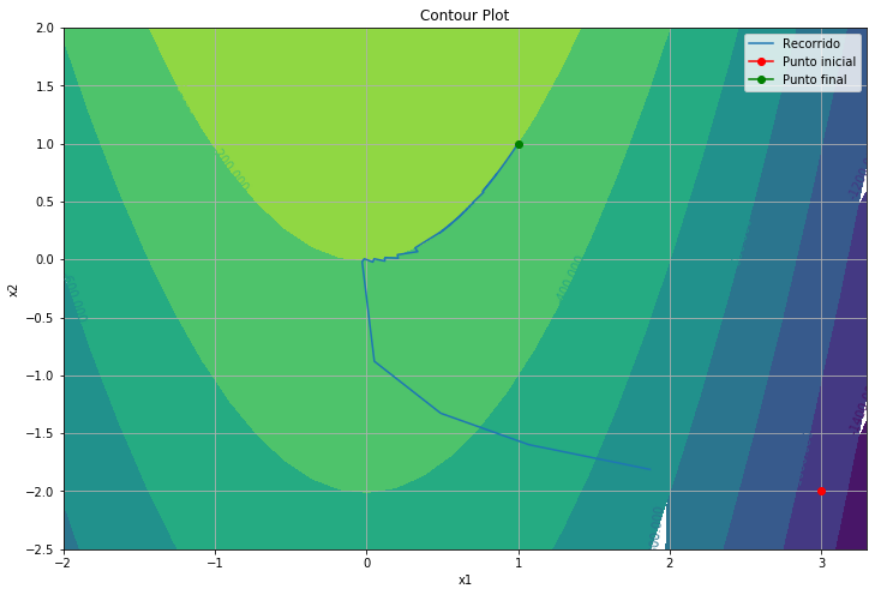
\includegraphics[scale=0.25]{3.png}
    \caption{Gráfico de contornos y convergencia para tamaño de paso por Backtracking}
    \label{k}
\end{figure}

\subsection{Resultados para la función de Rosembrock, n=100}

\begin{table}[H]
\begin{tabular}{@{}llll@{}}
k & $||x\_{k+1}-x_k||$ & $||\nabla f(x_k)||$ & $f(x_k)$ \\
1  &  6.027981E-01 &  1.025208E+03   &  6.654000E+02  \\
2  &  3.678791E-01 &  2.666164E+02   &  2.255963E+02  \\
3  &  2.102711E-01 &  6.223275E+01   &  1.426170E+02  \\
10000  &  5.010135E-07 &  2.619041E-04   &  1.052182E+02 \\
10001  &  5.040273E-07 &  2.615473E-04   &  1.052183E+02  \\
10002  &  5.074632E-07 &  2.611783E-04   &  1.052183E+02
\end{tabular}
\caption{Cuadro comparativo de los criterios de paro y convergencia de la función con tamaño de paso adaptable}
\end{table}

\begin{table}[H]
\begin{tabular}{@{}llll@{}}
k & $||x\_{k+1}-x_k||$ & $||\nabla f(x_k)||$ & $f(x_k)$ \\
1  &  1.277631E+00 &  9.491898E+02   &  1.924941E+03  \\
2  &  2.260324E+00 &  5.317003E+02   &  1.183481E+03  \\
3  &  1.078246E+00 &  8.278282E+02   &  1.212234E+03  \\
10000  &  4.170223E-07 &  2.331660E-04   &  4.815531E-08 \\
10001  &  4.043511E-07 &  2.333264E-04   &  4.808871E-08  \\
10002  &  3.942199E-07 &  2.329568E-04   &  4.802375E-08
\end{tabular}
\caption{Cuadro comparativo de los criterios de paro y convergencia de la función con tamaño de paso fijo}
\end{table}


\begin{table}[H]
\begin{tabular}{@{}llll@{}}
k & $||x\_{k+1}-x_k||$ & $||\nabla f(x_k)||$ & $f(x_k)$ \\
1  &  1.277631E+00 &  9.491898E+02   &  1.924941E+03  \\
2  &  2.260324E+00 &  5.317003E+02   &  1.183481E+03  \\
3  &  1.078246E+00 &  8.278282E+02   &  1.212234E+03  \\
10000  &  4.170223E-07 &  2.331660E-04   &  4.815531E-08 \\
10001  &  4.043511E-07 &  2.333264E-04   &  4.808871E-08  \\
10002  &  3.942199E-07 &  2.329568E-04   &  4.802375E-08
\end{tabular}
\caption{Cuadro comparativo de los criterios de paro y convergencia de la función con tamaño de paso por backtracking}
\end{table}

\subsection{}

\subsection{Resultados para la función de Wood}

\begin{table}[H]
\begin{tabular}{@{}llll@{}}
k & $||x\_{k+1}-x_k||$ & $||\nabla f(x_k)||$ & $f(x_k)$ \\
1  &  1.520915E+00 &  1.639713E+04   &  1.019200E+04  \\
2  &  1.064475E+00 &  4.969228E+03   &  2.672898E+03  \\
3  &  7.732140E-01 &  1.521797E+03   &  7.484454E+02  \\
10000  &  4.225988E-05 &  2.138291E-02   &  1.563470E-03 \\
10001  &  3.914430E-05 &  1.982988E-02   &  -4.854982E-03  \\
10002  &  4.214118E-05 &  2.132221E-02   &  1.558644E-03
\end{tabular}
\caption{Cuadro comparativo de los criterios de paro y convergencia de la función con tamaño de paso adaptable}
\end{table}

\begin{table}[H]
\begin{tabular}{@{}llll@{}}
k & $||x\_{k+1}-x_k||$ & $||\nabla f(x_k)||$ & $f(x_k)$ \\
1  &  8.344961E-01 &  2.090938E+02   &  -7.464740E+01  \\
2  &  2.139071E-01 &  2.034307E+02   &  5.124507E+01  \\
3  &  9.193321E-02 &  4.149943E+01   &  1.520606E+01  \\
10000  &  1.394707E-10 &  6.982503E-08   &  -4.675136E-09 \\
10001  &  1.284017E-10 &  6.436736E-08   &  1.632233E-08  \\
10002  &  1.390694E-10 &  6.962422E-08   &  -4.661681E-09
\end{tabular}
\caption{Cuadro comparativo de los criterios de paro y convergencia de la función con tamaño de paso fijo}
\end{table}

\begin{table}[H]
\begin{tabular}{@{}llll@{}}
k & $||x\_{k+1}-x_k||$ & $||\nabla f(x_k)||$ & $f(x_k)$ \\
1  &  8.344961E-01 &  2.090938E+02   &  -7.464740E+01  \\
2  &  2.139071E-01 &  2.034307E+02   &  5.124507E+01  \\
3  &  9.193321E-02 &  4.149943E+01   &  1.520606E+01  \\
10000  &  1.394707E-10 &  6.982503E-08   &  -4.675136E-09 \\
10001  &  1.284017E-10 &  6.436736E-08   &  1.632233E-08  \\
10002  &  1.390694E-10 &  6.962422E-08   &  -4.661681E-09
\end{tabular}
\caption{Cuadro comparativo de los criterios de paro y convergencia de la función con tamaño de paso por backtracking}
\end{table}

\section{Conclusiones}

De los 3 modos de de obtención del tamaño de paso el que mejor se comporto fué el adaptable teniendo un menor número de iteraciónes y convergencia mucho mejor a los demás.

cabe recalcar que como se observa en los resultados no se pudo obtener buenos resultados usando el tamaño de paso calculado mediante backtracking.

Para la segunda función evaluada se observó que se el algoritmo se estancaba en un minimo local, puesto el vector final contenía un signo negativo en uno de sus componentes. Así teniendo en cuenta que se debe mejorar para poder salir de eso mínimos locales.

\end{document}
